\documentclass[12pt,oneside,a4paper]{article}
\usepackage{tikz}
\usetikzlibrary{arrows.meta,arrows}
\author{Siberia怒风}
\begin{document}
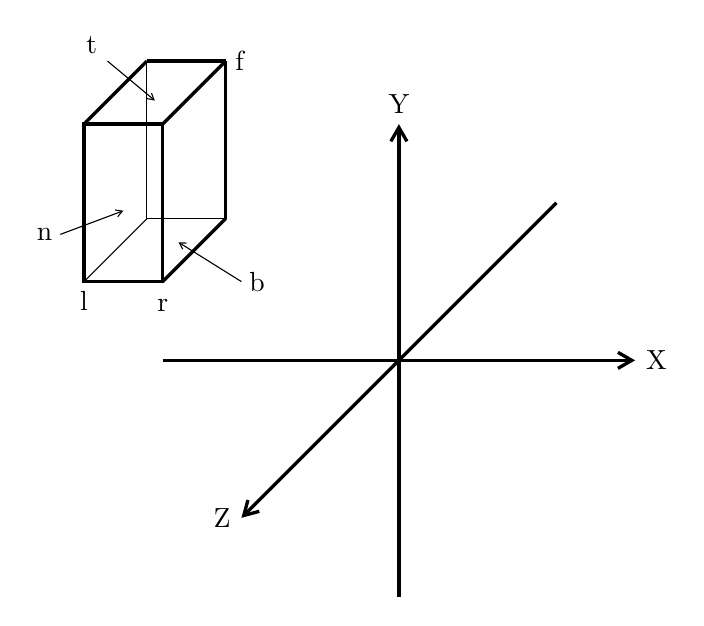
\begin{tikzpicture}
[>={Straight Barb[angle=60:1pt 4]},
myarrow/.style={
decoration={
markings,
mark=at position 0.5 with {\arrow {Straight Barb}};}
postaction = decorate}]
  \draw [->, very thick](-3,0) -- (3,0) node[right]{X};
  \draw [->, very thick](0,-3) -- (0,3) node[above]{Y};
  \draw [->, very thick](2,2) -- (-2,-2) node[left]{Z};
  \draw [very thick] (-4,1) rectangle (-3,3);
  \draw (-3.2,1.8) rectangle (-2.2,3.8);
  \draw [very thick] (-3.2,3.8) -- (-2.2,3.8);
  \draw [very thick] (-2.2,1.8) -- (-2.2,3.8);
  \draw (-4,1) -- (-3.2,1.8);
  \draw [very thick] (-3,1) -- (-2.2,1.8);
  \draw [very thick] (-4,3) -- (-3.2,3.8);
  \draw [very thick] (-3,3) -- (-2.2,3.8);
  \draw [->] (-4.3,1.6) -- (-3.5,1.9);
  \draw (-4.5,1.6) node {n};
  \draw [->] (-3.7,3.8) -- (-3.1,3.3);
  \draw (-3.9,4.0) node {t};
  \draw [->] (-2.0,1.0) -- (-2.8,1.5);
  \draw (-1.8,1.0) node {b};
  \node [below] at (-4,1) {l};
  \draw (-3,0.7) node {r};
  \node [right] at (-2.2,3.8) {f};
\end{tikzpicture}
\end{document}